\documentclass[12pt]{article}

% Imports
\usepackage{hyperref}
\usepackage[margin=0.5in]{geometry}
\usepackage{ctable}
\usepackage{array}
\usepackage{graphicx}

% Paragraph spacing
\setlength{\parindent}{0em}
\setlength{\parskip}{0.5em}

% Default font
\renewcommand*{\familydefault}{\sfdefault}

% table lines
\newcolumntype{?}{!{\vrule width 1pt}}

% hyperlinks
\hypersetup{
  breaklinks=true,  % so long urls are correctly broken across lines
  colorlinks=true,
  urlcolor=blue,
  linkcolor=red,
  citecolor=red,
 }

\begin{document}

% Header info
\textbf{CS 291 - PERSONAL GENOMICS FOR BIOINFORMATICIANS}

\section*{Problem Set 1 - Introduction to human genomes}

All homework should be sent to mgymrek@ucsd.edu with subject line [CSE291 PS1:LASTNAME] by the beginning of class on \textbf{Tuesday, January 10}.

\subsection*{Objectives}
\begin{itemize}
\item Review human genetics concepts.
\item Get comfortable with standard file formats and tools for analyzing genomes.
\end{itemize}

%\subsection*{You will need} % TODO maybe I can put this all on comet on education allocation? then will already be installed
%\begin{itemize}
%\item Access to a UNIX terminal.
%\item Download PS1 data: \href{https://gymreklab.github.io/teaching/personal\_genomics/ps1\_introduction.html}{https://gymreklab.github.io/teaching/personal\_genomics/ps1\_introduction.html}. % Genome file, bed file
%\item Download and install \texttt{tabix} and \texttt{bedtools}.
%\end{itemize}

\subsection*{Exercises}
\begin{enumerate}

\item How many chromosomes does a typical human have? Remember to consider copies from both parents.

\item Approximately what percent of the genome consists of protein coding genes?

\item Identify the labeled components of a typical gene depicted below. Options are: exon, intron, 5'UTR, 3'UTR, splice site, promoter/regulatory region.
\begin{figure}[h!]
\centering
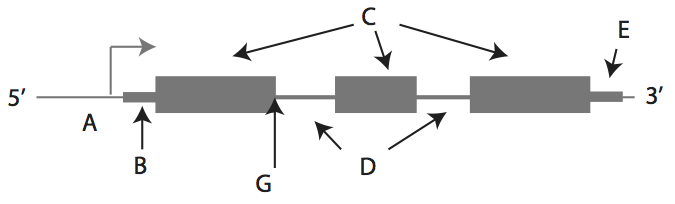
\includegraphics[width=200px]{pset1gene.png}
\end{figure}

\item You see a gene with the following coding sequence: XXX TODO. Give (1) the sequence of the transcribed mRNA and (2) the amino acid sequence of the translated protein.

\item A mutation occurs in the gene from the previous question, resulting in a sequence XXX TODO. What is the amino acid sequence of the new protein? This is known as a \emph{synonymous mutation}.

\item A different mutation occurs in the same gene, now resulting in a sequence XXX TODO. What is the amino acid sequence of the new protein? This is known as a \emph{missense mutation}.

\item What modes of inheritance are consistent with the following pedigree? Name an example human condition that follows this mode of inheritance.
\begin{figure}[h!]
\centering
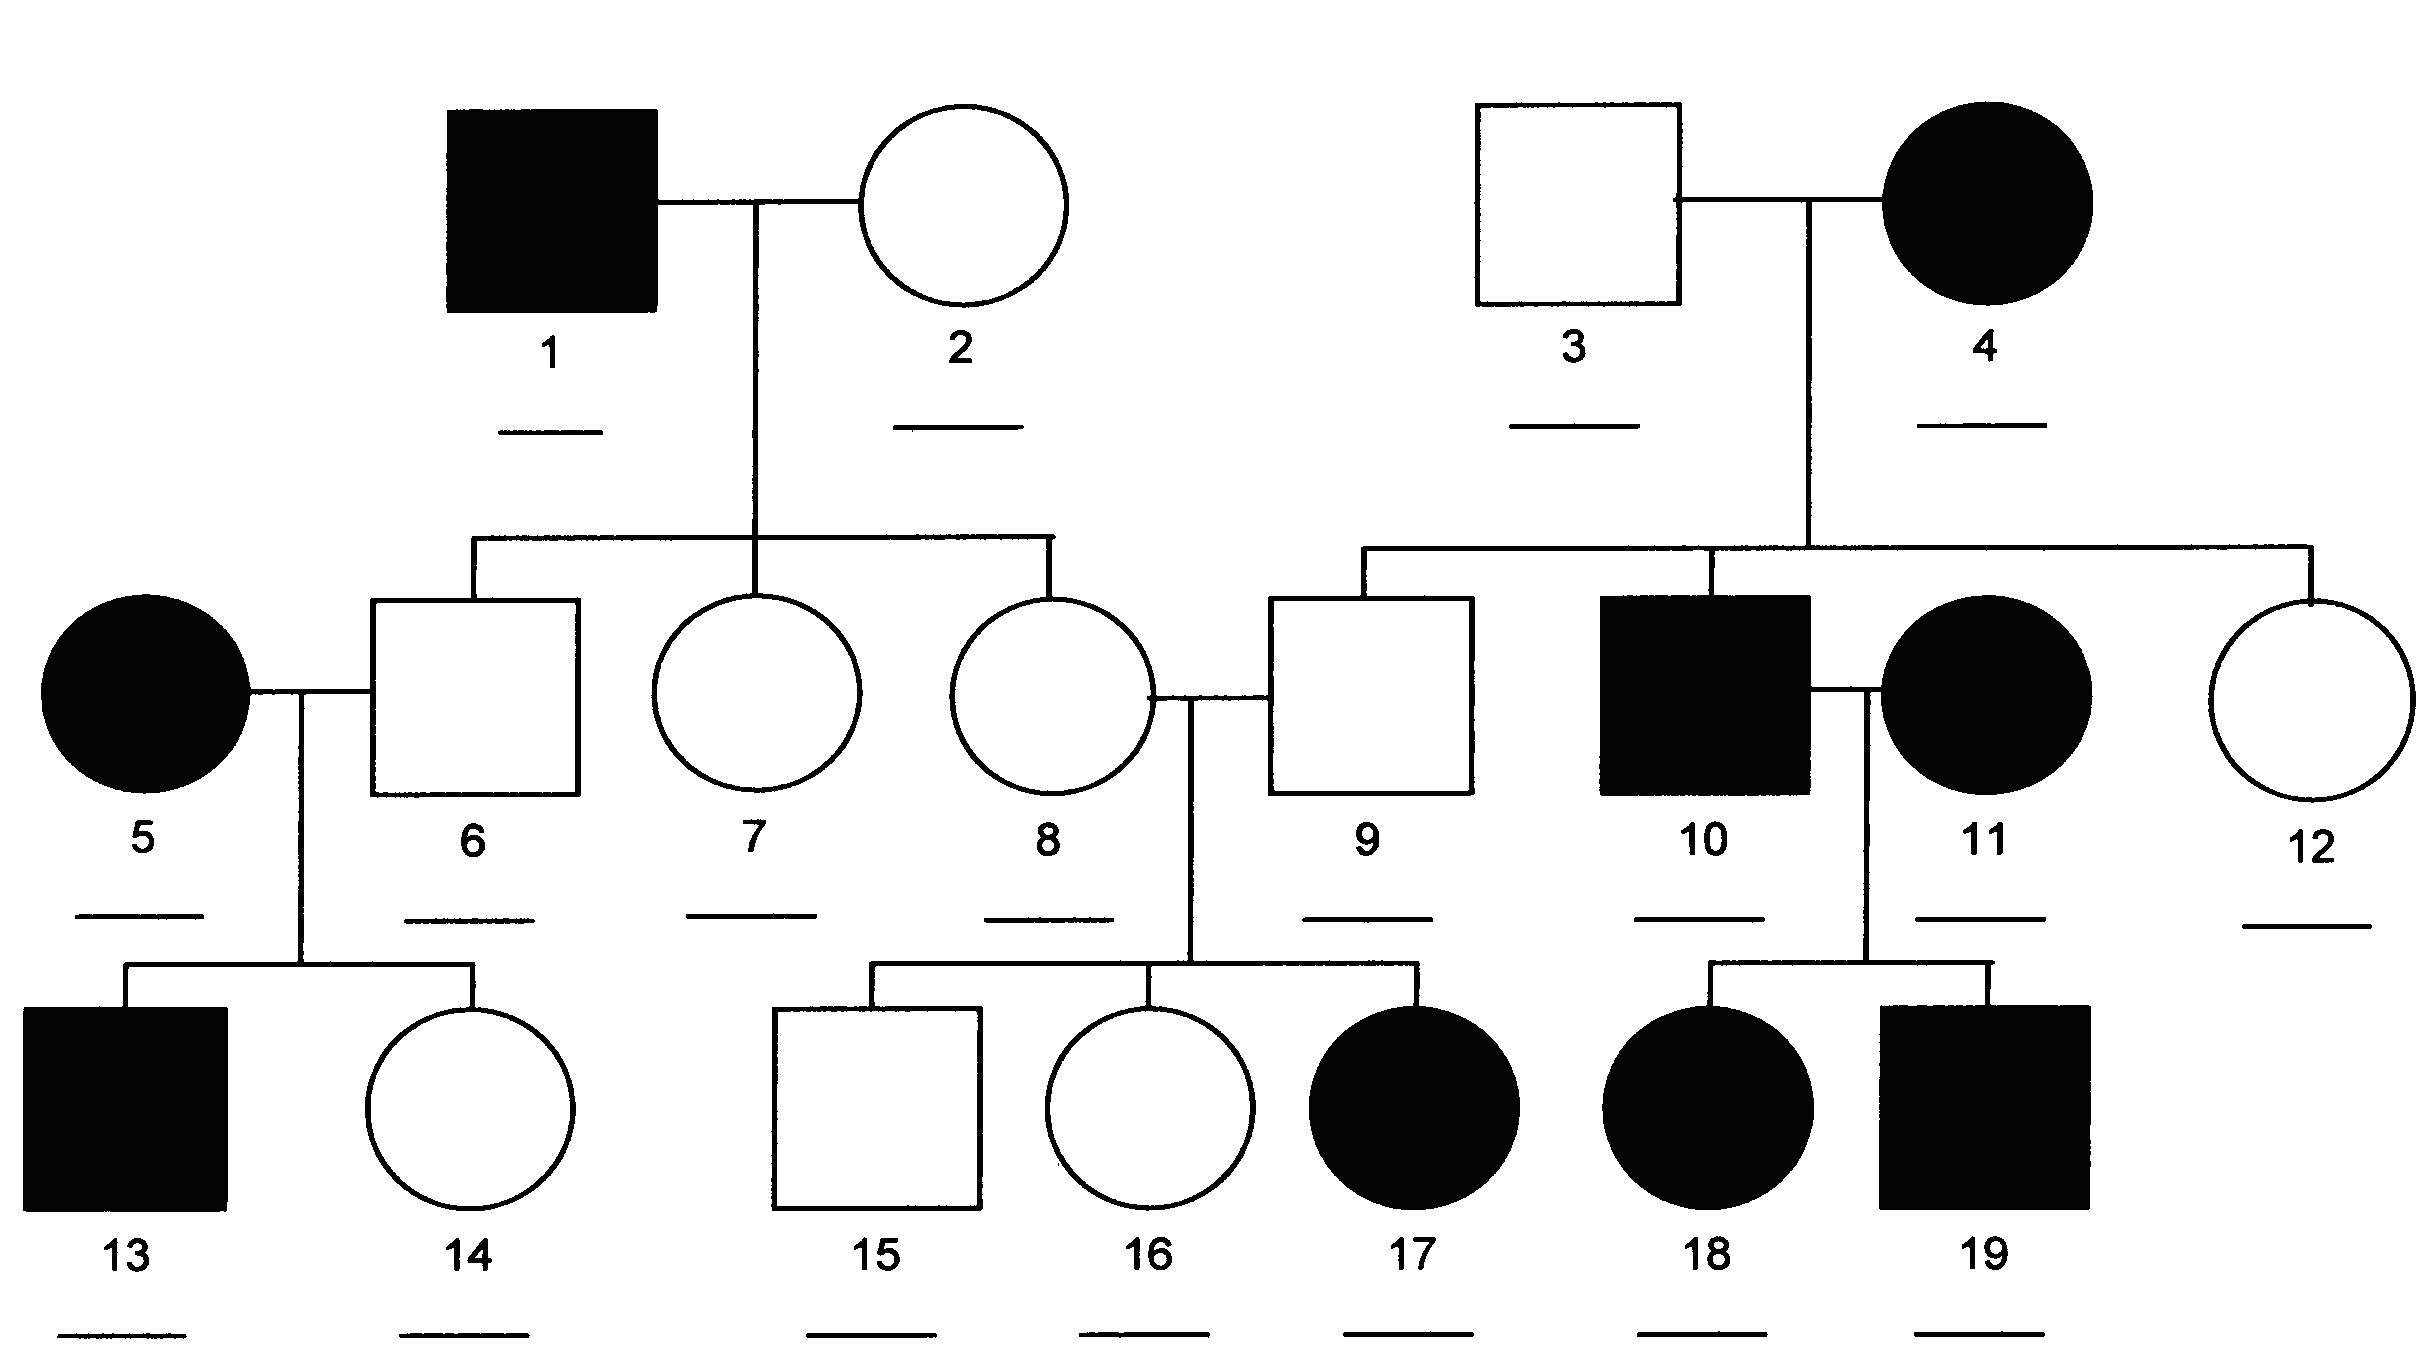
\includegraphics[width=150px]{pset1recessive.png}
\end{figure}

\item What modes of inheritance are consistent with the following pedigree? Name an example human condition that follows this mode of inheritance.

\begin{figure}[h!]
\centering
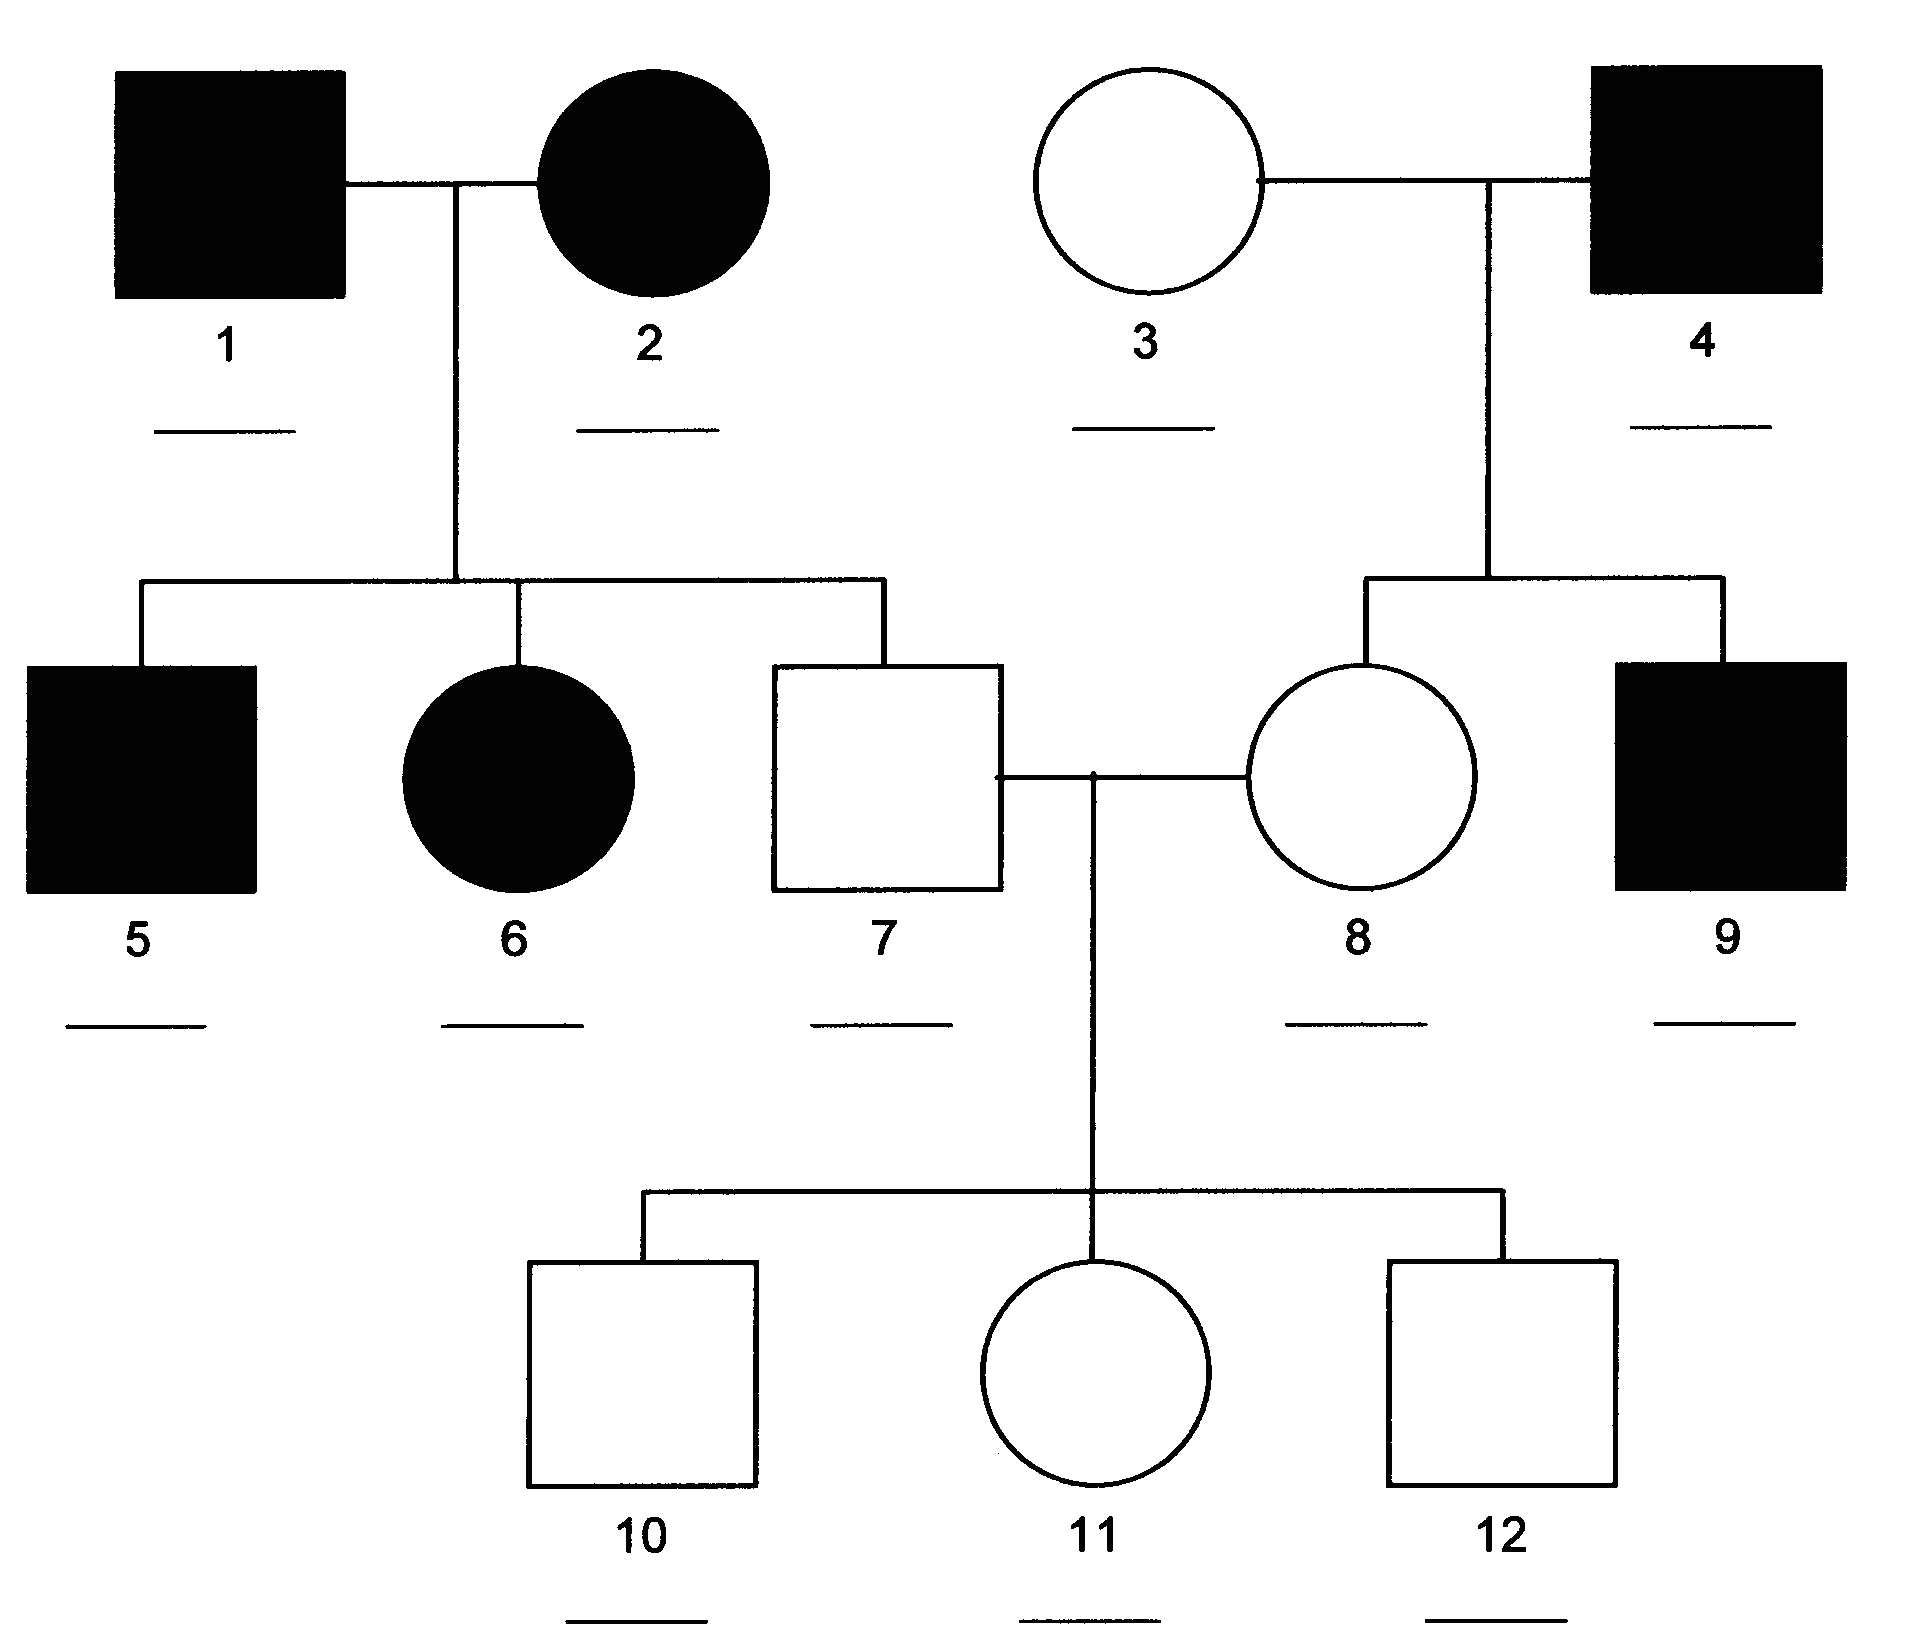
\includegraphics[width=150px]{pset1dominant.png}
\end{figure}

\item Download \href{https://gymreklab.github.io/teaching/personal\_genomics/ps1\_introduction.html}{PS1 data} from the course website. First, we'll get familiar with the VCF file format. For full details of VCF format, see . %TODO name of VCF file? if on server, don't need to download
\begin{itemize}
\item Lines at the top of the file marked with ``\#\#'' indicate the header. What build of the human reference genome is used in this file?
\item Look at the first entry (XX TODO). What is the reference allele? What is the alternate allele?
\item What is the individual's genotype at this position (e.g. AG, GG, etc.).
\end{itemize}

\item This individual comes to the hospital with a blood clot. The doctor would like to treat the patient with warfarin, but is trying to figure out the correct dose. Studies have shown that individuals with XXX TODO tell this story. We would like to find out whether this patient is at risk.

VCF genomes can be quite large (the VCF file for the ExAC dataset is more than 1TB!). If we want to query a specific location of the genome, it would be inefficient to scan the entire file. \texttt{tabix} offers utilities to build an index for VCF (and other) files to enable quick access to a specific location. Use the tabix utility to index the VCF file with the following command:
 % TODO code box with command

Now, use the tabix utility to pull out our SNP of interest:
% TODO code box with command

What should the doctor do?

\item The doctor now suspects the patient might have a genetic disorder known to be caused by mutations in the gene XXX TODO. We would like to determine whether the individual has any mutations in the protein-coding sequence of this gene. Luckily, we have a file XX TODO listing the genomic coordinates of each exon in this gene. This is an example of a BED file, which gives the chromosome, start coordinate, and end coordinate of each interval.

Intersecting genomic intervals is an extremely common task. \texttt{bedtools} contains many utilities for working with BED files. Use the \texttt{intersectBed} utility to look at all variants falling within the given intervals.
% TODO code box with command.

How many did you find? 

\end{enumerate}

\end{document}